
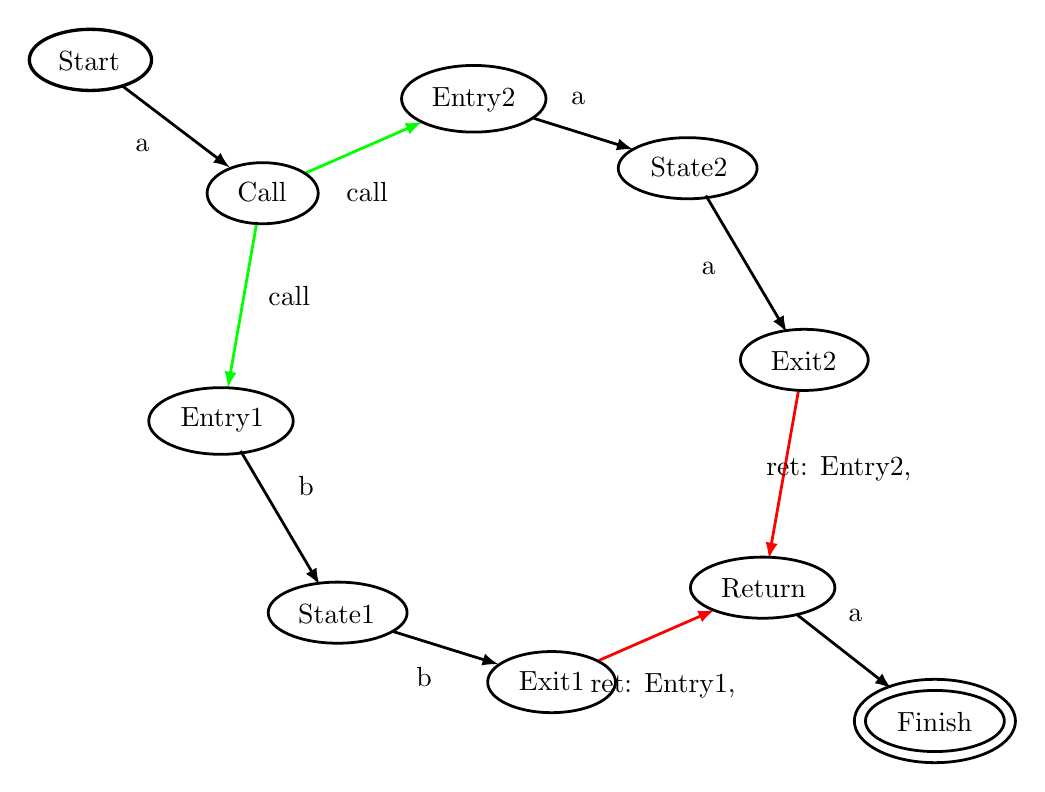
\begin{tikzpicture}[>=latex,line join=bevel,]
  \pgfsetlinewidth{1bp}
%%
\pgfsetcolor{black}
  % Edge: Exit2 -> Return
  \pgfsetcolor{red}
  \draw [->] (278.88bp,134.9bp) .. controls (276.63bp,122.15bp) and (272.82bp,100.54bp)  .. (268.21bp,74.402bp);
  \definecolor{strokecol}{rgb}{0.0,0.0,0.0};
  \pgfsetstrokecolor{strokecol}
  \draw (293.43bp,106.69bp) node {ret: Entry2, };
  % Edge: Call -> Entry1
  \pgfsetcolor{green}
  \draw [->] (83.911bp,195.7bp) .. controls (81.716bp,183.15bp) and (78.025bp,162.04bp)  .. (73.465bp,135.96bp);
  \definecolor{strokecol}{rgb}{0.0,0.0,0.0};
  \pgfsetstrokecolor{strokecol}
  \draw (95.57bp,168.88bp) node {call};
  % Edge: State2 -> Exit2
  \draw [->] (245.56bp,205.17bp) .. controls (251.84bp,194.54bp) and (261.78bp,177.72bp)  .. (274.65bp,155.96bp);
  \draw (246.53bp,178.92bp) node {a};
  % Edge: Exit1 -> Return
  \pgfsetcolor{red}
  \draw [->] (207.02bp,37.797bp) .. controls (216.49bp,41.931bp) and (228.52bp,47.183bp)  .. (248.66bp,55.978bp);
  \definecolor{strokecol}{rgb}{0.0,0.0,0.0};
  \pgfsetstrokecolor{strokecol}
  \draw (230.14bp,28.836bp) node {ret: Entry1, };
  % Edge: State1 -> Exit1
  \draw [->] (132.99bp,48.215bp) .. controls (141.61bp,45.526bp) and (151.82bp,42.344bp)  .. (170.95bp,36.381bp);
  \draw (144.1bp,31.817bp) node {b};
  % Edge: Start -> Call
  \draw [->] (35.215bp,244.83bp) .. controls (43.915bp,238.22bp) and (55.982bp,229.06bp)  .. (74.122bp,215.28bp);
  \draw (42.681bp,223.09bp) node {a};
  % Edge: Call -> Entry2
  \pgfsetcolor{green}
  \draw [->] (101.2bp,213.16bp) .. controls (110.62bp,217.28bp) and (122.94bp,222.67bp)  .. (143.35bp,231.59bp);
  \definecolor{strokecol}{rgb}{0.0,0.0,0.0};
  \pgfsetstrokecolor{strokecol}
  \draw (123.61bp,206.34bp) node {call};
  % Edge: Entry2 -> State2
  \draw [->] (183.56bp,232.98bp) .. controls (191.6bp,230.46bp) and (200.89bp,227.56bp)  .. (219.32bp,221.79bp);
  \draw (199.55bp,239.91bp) node {a};
  % Edge: Entry1 -> State1
  \draw [->] (78.069bp,113.22bp) .. controls (84.301bp,102.65bp) and (93.768bp,86.578bp)  .. (106.44bp,65.076bp);
  \draw (101.64bp,100.58bp) node {b};
  % Edge: Return -> Finish
  \draw [->] (278.49bp,54.169bp) .. controls (285.83bp,48.432bp) and (295.42bp,40.929bp)  .. (312.27bp,27.748bp);
  \draw (299.35bp,54.115bp) node {a};
  % Node: Entry2
\begin{scope}
  \definecolor{strokecol}{rgb}{0.0,0.0,0.0};
  \pgfsetstrokecolor{strokecol}
  \draw (162bp,240bp) ellipse (26bp and 12bp);
  \draw (161.97bp,239.74bp) node {Entry2};
\end{scope}
  % Node: Finish
\begin{scope}
  \definecolor{strokecol}{rgb}{0.0,0.0,0.0};
  \pgfsetstrokecolor{strokecol}
  \draw (328bp,16bp) ellipse (25bp and 11bp);
  \draw (328bp,16bp) ellipse (29bp and 15bp);
  \draw (327.93bp,15.5bp) node {Finish};
\end{scope}
  % Node: Exit1
\begin{scope}
  \definecolor{strokecol}{rgb}{0.0,0.0,0.0};
  \pgfsetstrokecolor{strokecol}
  \draw (190bp,30bp) ellipse (23bp and 11bp);
  \draw (190.1bp,30.411bp) node {Exit1};
\end{scope}
  % Node: State2
\begin{scope}
  \definecolor{strokecol}{rgb}{0.0,0.0,0.0};
  \pgfsetstrokecolor{strokecol}
  \draw (239bp,215bp) ellipse (25bp and 11bp);
  \draw (239.46bp,215.48bp) node {State2};
\end{scope}
  % Node: Exit2
\begin{scope}
  \definecolor{strokecol}{rgb}{0.0,0.0,0.0};
  \pgfsetstrokecolor{strokecol}
  \draw (281bp,146bp) ellipse (23bp and 11bp);
  \draw (280.77bp,145.61bp) node {Exit2};
\end{scope}
  % Node: Start
\begin{scope}
  \definecolor{strokecol}{rgb}{0.0,0.0,0.0};
  \pgfsetstrokecolor{strokecol}
  \draw [very thick] (24bp,254bp) ellipse (22bp and 11bp);
  \draw (23.5bp,253.73bp) node {Start};
\end{scope}
  % Node: State1
\begin{scope}
  \definecolor{strokecol}{rgb}{0.0,0.0,0.0};
  \pgfsetstrokecolor{strokecol}
  \draw (113bp,55bp) ellipse (25bp and 11bp);
  \draw (112.63bp,54.56bp) node {State1};
\end{scope}
  % Node: Entry1
\begin{scope}
  \definecolor{strokecol}{rgb}{0.0,0.0,0.0};
  \pgfsetstrokecolor{strokecol}
  \draw (71bp,124bp) ellipse (26bp and 12bp);
  \draw (71.453bp,124.45bp) node {Entry1};
\end{scope}
  % Node: Call
\begin{scope}
  \definecolor{strokecol}{rgb}{0.0,0.0,0.0};
  \pgfsetstrokecolor{strokecol}
  \draw (86bp,206bp) ellipse (20bp and 11bp);
  \draw (85.784bp,206.42bp) node {Call};
\end{scope}
  % Node: Return
\begin{scope}
  \definecolor{strokecol}{rgb}{0.0,0.0,0.0};
  \pgfsetstrokecolor{strokecol}
  \draw (266bp,64bp) ellipse (26bp and 11bp);
  \draw (266.32bp,63.69bp) node {Return};
\end{scope}
%
\end{tikzpicture}
